\documentclass[11pt,a4paper]{article}
\usepackage[T1]{fontenc}
\usepackage[utf8]{inputenc}
\usepackage{lmodern,microtype,amsmath,graphicx,booktabs}
\usepackage[margin=24mm,headheight=15pt]{geometry}
\usepackage{xcolor,parskip,fancyhdr,hyperref}
\definecolor{ink}{HTML}{192532}\definecolor{navy}{HTML}{1F4874}\definecolor{muted}{HTML}{52677B}
\hypersetup{colorlinks=true,urlcolor=navy,pdftitle={Big Data, Sustainability and Governance},pdfauthor={Jacques Girard, Gauthier Jeannin, Corentin Leconte, Alexandre O'Neill, Enzo Touak, Hugo Wei}}
\pagestyle{fancy}\fancyhf{}\fancyhead[L]{\footnotesize\color{muted} RESEARCH ARCHIVE / INTERDISCIPLINARY REVIEW}\fancyhead[R]{\footnotesize\color{muted} H. WEI}\fancyfoot[C]{\footnotesize\thepage}
\renewcommand{\headrulewidth}{0.35pt}
\newcommand{\sect}[1]{\par\vspace{3mm}\noindent{\large\bfseries\color{navy}#1}\par\vspace{1mm}}
\begin{document}
{\color{navy}\sffamily\bfseries\small RESEARCH SYNOPSIS\quad / \quad EDITORIAL EDITION 2026}\par\vspace{5mm}
{\fontsize{28}{33}\selectfont\bfseries\color{ink} Big Data, Sustainability\\ and Governance}\par\vspace{4mm}
{\large Environmental impacts, data ethics, public value, and institutional design}\par\vspace{5mm}
\hrule\vspace{4mm}
{\small \textbf{Original group report:} \emph{Big Data : comment l'emp\^echer de devenir un cheval de Troie} (ESCP Business School, 2023).\\
\textbf{Authors:} Jacques Girard, Gauthier Jeannin, Corentin Leconte, Alexandre O'Neill, Enzo Touak, Hugo Wei.\\
\textbf{Academic supervisor:} Caroline Verzat. \textbf{Format:} Interdisciplinary review and interviews.}\par
\sect{Central question}
Under what technical, economic and institutional conditions can large-scale data analysis create social value without externalizing costs to the environment, privacy, fair competition or democratic accountability?
\sect{Research structure}
The original collaborative study connected four strands: (i) environmental costs and mitigation options in data collection, processing and storage; (ii) privacy, ethical use and the legal basis for data governance; (iii) applications in sports analytics, medicine and business; and (iv) data stewardship and the potential role of shared governance. It combined a literature review with interviews carried out for the student project.
\begin{figure}[ht]
\centering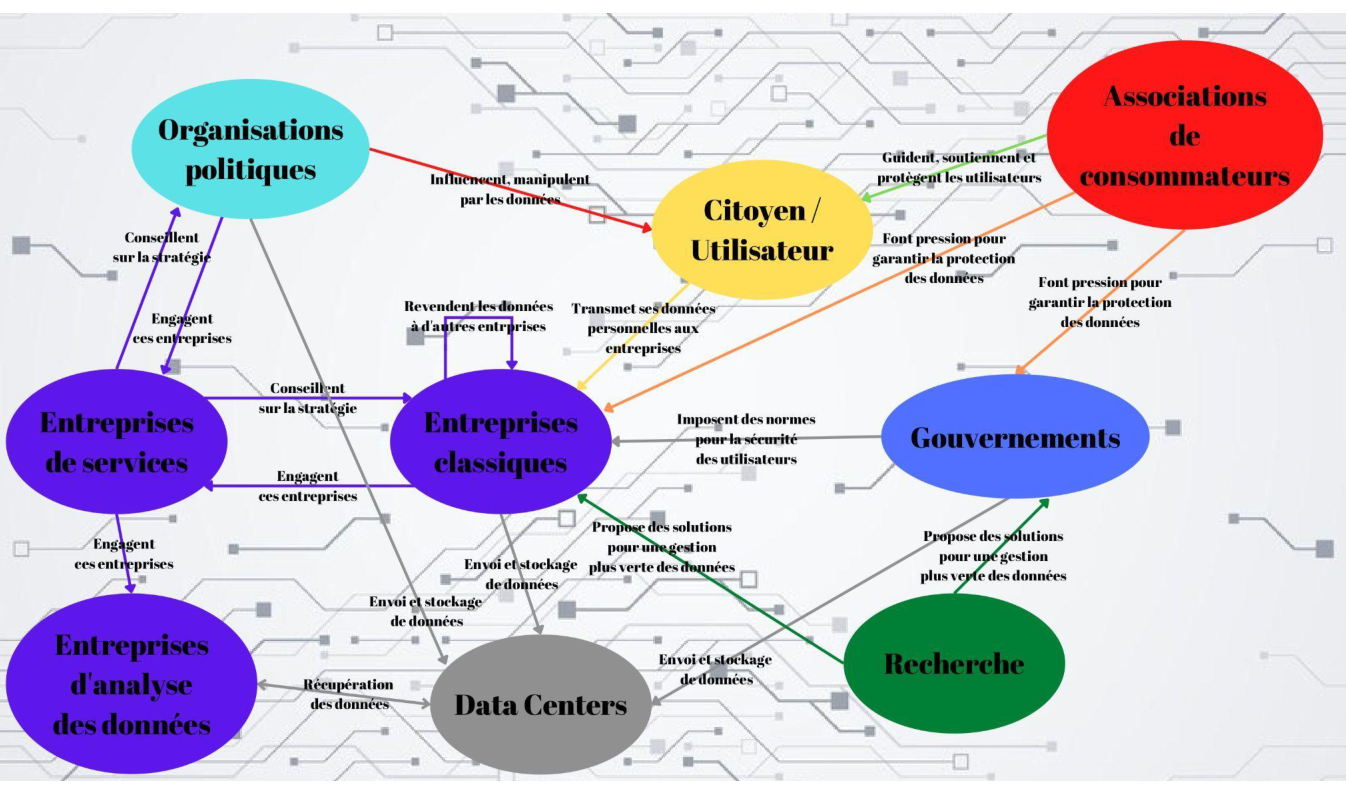
\includegraphics[width=.94\textwidth]{stakeholder-map.png}
\caption{Original stakeholder map from the 2023 group report, showing the relationships among citizens, governments, data centres, research and service providers. Reproduced here as an archival figure.}
\end{figure}
\sect{Updated factual context (sources and years explicit)}
The International Energy Agency estimated that data centres used around \textbf{415 TWh} of electricity worldwide in \textbf{2024}, approximately \textbf{1.5\%} of total global electricity consumption. Its \emph{Energy and AI} base-case projection published in \textbf{2025} put 2030 data-centre demand at around \textbf{945 TWh}; this is a scenario projection, not observed 2030 consumption.\footnote{IEA, \emph{Energy and AI}, executive summary (2025): \url{https://www.iea.org/reports/energy-and-ai/executive-summary}.}

The European Union's AI Act entered into force in August 2024 and applies in stages. Some provisions began applying in 2025 and 2026; other requirements have later implementation dates. This regulatory landscape is distinct from the GDPR and should not be described as a single complete set of rules already in effect.\footnote{Council of the European Union, \emph{Artificial intelligence act}: \url{https://www.consilium.europa.eu/en/policies/artificial-intelligence-act/}.}
\sect{Analytical lessons}
\begin{enumerate}\setlength\itemsep{3pt}
\item \textbf{Measure impacts in the right units.} Distinguish electricity demand, energy mix, lifecycle emissions, water use and local grid constraints. An estimate for data centres cannot automatically be generalized to all digital technology.
\item \textbf{Make dates and assumptions visible.} Retrospective studies must separate measurements from scenarios and retain the date of each estimate. Numbers drawn from the original 2023 report should not be quoted as current 2026 measurements.
\item \textbf{Treat governance as system design.} Privacy protection, access rights, accountability and incentives shape which data-driven applications provide genuine public value.
\item \textbf{Separate expert interviews from public evidence.} Interview statements are contextual testimony rather than independently verified factual claims, especially when concerning named third parties.
\end{enumerate}
\sect{Provenance and publication scope}
The original document is a \emph{team-produced student research report}. The figure above preserves one of its original visual elements. The present synopsis revisits its framing and cites newer primary sources, but does not revalidate all numerical claims in the 94-page historical manuscript. Interviews, original image credits and other contributors' publication permissions require review before the full text is distributed publicly. This public-facing note intentionally does not reproduce interview transcripts.
\par\vspace{3mm}
\hrule\vspace{2mm}{\footnotesize\color{muted} Editable LaTeX source and the original stakeholder diagram accompany this publication note. This is a curated synopsis, not a peer-reviewed journal article or a full rewritten version of the original report.}
\end{document}
